\documentclass{book}
\usepackage{graphicx}                              %for PNG images (pdflatex)
\usepackage[linkbordercolor={1.0 1.0 0.0}]{hyperref} %for \url tag
\usepackage{color}                                 %for defining custom colors
\usepackage{framed}                                %for shaded and framed paragraphs
\usepackage{textcomp}                              %for various symbols, e.g. Registered Mark
\usepackage{geometry}                              %for defining page size
\usepackage{longtable}                             %for breaking tables
%
\geometry{verbose,a4paper,tmargin=2.5cm,bmargin=2.5cm,lmargin=2.5cm,rmargin=2cm}
\hypersetup{
  pdfauthor = {Zsombor Nagy},
  pdftitle = {Documentation of the ARC storage system},
  pdfsubject = {Paper subject},
  pdfkeywords = {Paper,keyword,comma-separated},
  pdfcreator = {PDFLaTeX with hyperref package},
  pdfproducer = {PDFLaTeX}
}
%
\bibliographystyle{IEEEtran}                       %a nice bibliography style
%
\def\efill{\hfill\nopagebreak}%
\hyphenation{Nordu-Grid}
\setlength{\parindent}{0cm}
\setlength{\FrameRule}{1pt}
\setlength{\FrameSep}{8pt}
\addtolength{\parskip}{5pt}
\renewcommand{\thefootnote}{\fnsymbol{footnote}}
\renewcommand{\arraystretch}{1.3}
\newcommand{\dothis}{\colorbox{shadecolor}}
\newcommand{\ngdl}{\url{http://ftp.nordugrid.org/download}~}
\definecolor{shadecolor}{rgb}{1,1,0.6}
\definecolor{salmon}{rgb}{1,0.9,1}
\definecolor{bordeaux}{rgb}{0.75,0.,0.}
\definecolor{cyan}{rgb}{0,1,1}
%
%----- DON'T CHANGE HEADER MATTER
\hyphenation{preserve-Original}
\begin{document}
\def\today{\number\day/\number\month/\number\year}

\begin{titlepage}

\begin{tabular}{rl}
\resizebox*{3cm}{!}{
\includegraphics{ng-logo.png}}
&\parbox[b]{2cm}{\textbf \it {\hspace*{-1.5cm}NORDUGRID\vspace*{0.5cm}}}
\end{tabular}

\hrulefill

%-------- Change this to NORDUGRID-XXXXXXX-NN

{\raggedleft NORDUGRID-TECH-17\par}

{\raggedleft \today\par}

\vspace*{2cm}

%%%%---- The title ----
{\centering \textsc{\Large Documentation of the ARC storage system}\Large \par}
\vspace*{0.5cm}
    
%%%%---- A subtitle, if necessary ----
{\centering \textit{\large First prototype status and plans}\large \par}
    
\vspace*{1.5cm}
%%%%---- A list of authors ----
    {\centering \large Zsombor Nagy\footnote{zsombor@niif.hu} \large \par}
    {\centering \large Jon Nilsen\footnote{j.k.nilsen@usit.uio.no} \large \par}
    {\centering \large Salman Zubair Toor \footnote{salman.toor@it.uu.se} \large \par}
\end{titlepage}

\tableofcontents                          %Comment if use article style
\newpage

\renewcommand{\thefootnote}{\arabic{footnote}}


\chapter{Design Overview}
\label{cha:overview}


The ARC storage system is a distributed system for storing replicated \emph{file}s on several file storage nodes and manage them in a global namespace.  The files can be grouped into \emph{collection}s (a concept very similar to directories in the common file systems), and a collection can contain sub-collections and sub-sub-collections in any depth. There is a dedicated \emph{root collection} to gather all collections to the global namespace. This hierarchy of collections and files can be referenced using \emph{Logical Name}s (\emph{LN}s). The users can use this global namespace as they were using a local filesystem. Files can be transfered by multiple transfer protocols, and the client side tools hide this from the user. The replicas of the files are stored on different storage nodes. A storage node here is a network-accessible computer having storage space to share, and a storage element service running (e.g.~HTTP(S), FTP(S), GridFTP, ByteIO\footnote{OGSA ByteIO Working Group (BYTEIO-WG), \url{https://forge.gridforum.org/projects/byteio-wg/}}, etc.). For each storage node one of the services of the ARC storage system is needed to manage it and to integrate it into the system. There is a way on the client side to access third-party storage solutions through the namespace of the ARC storage system. The main services of the storage system are the following (see Figure~\ref{fig:services}):
\begin{itemize}
    \item the \textbf{A-Hash} service, which is a replicated database which is used by the Librarian to store metadata;
    \item the \textbf{Librarian} service, which handles the metadata and hierarchy of collections and files, the location of replicas, and health data of the Shepherd services, using the A-Hash as database;
    \item the \textbf{Bartender} service, which provides a high-level interface for the users and for other services;
    \item the \textbf{Shepherd} service, which manages storage element services, and provides a simple interface for storing files on storage nodes.
\end{itemize}

\begin{figure}[ht]
\centering{{\scalebox{0.9}{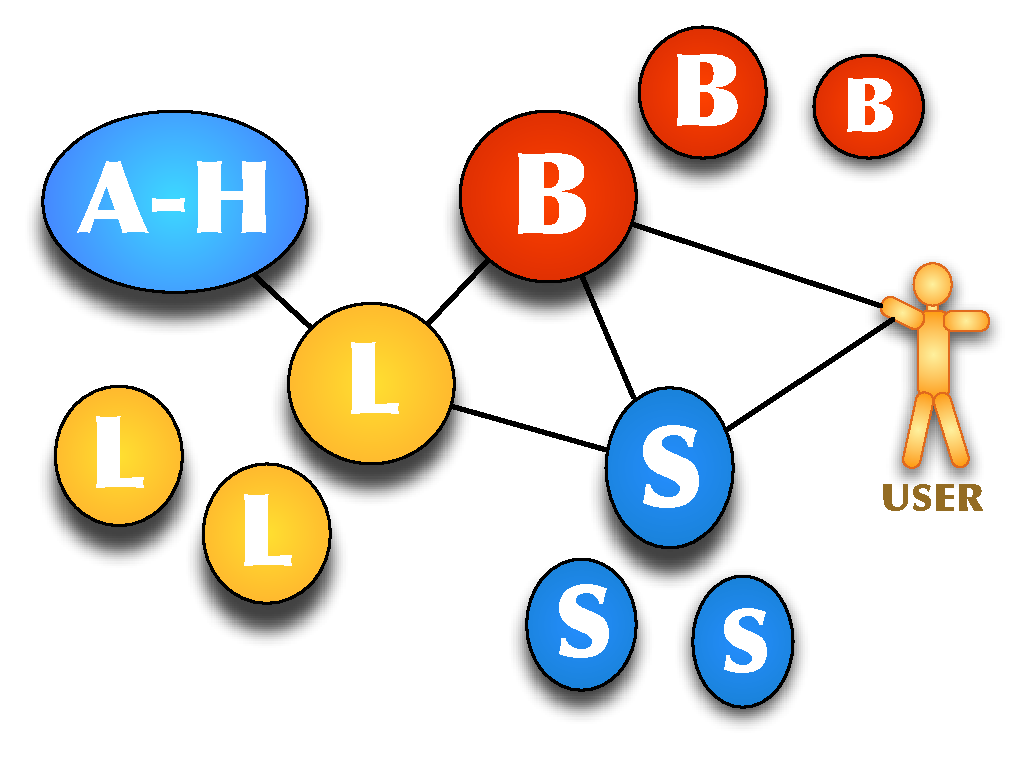
\includegraphics{arc-storage-services.pdf}}}
\caption{\label{fig:services}The components of the ARC storage: the \textbf{A-H}ash service, the \textbf{L}ibrarian service, the \textbf{B}artender service and the \textbf{S}hepherd service.}}
\end{figure}

\section{Files and collections} % (fold)
\label{sec:files_and_collections}

The storage system is capable of storing files which can be grouped in collections and sub-collections, etc.
Every file and collection has a unique ID in the sysem called the \emph{GUID}. Compared to the well-known structure of local file systems, these GUIDs are very similar to the concept of \emph{inode}s. And as a directory on a local filesystem is basically just a list of name and inode pairs, a collection on the ARC storage is just a list of name and GUID pairs. There is a dedicated collection which is the \emph{root collection}. This makes the namespace of the ARC storage system a hierarchical namespace where you can start at the root collection, and go to sub-collections and sub-sub-collections to get to a file. This path is called the \emph{Logical Name} (LN). For example if there is a sub-collection called \verb!saturn! in the root collection, and there is a file called \verb!rings! in this sub-collection, then the LN of this file is \verb!/saturn/rings!.

Besides the Logical Names we can refer to a file or collection by simply its GUID, or we can use GUIDs and Logical Names together, as seen on Figure~\ref{fig:namespace}.

The full syntax of Logical Names is \verb#/[path]# or \verb#<GUID>[/<path>]# where [...] indicates optional parts.

\begin{figure}[ht]
\centering{{\scalebox{0.7}{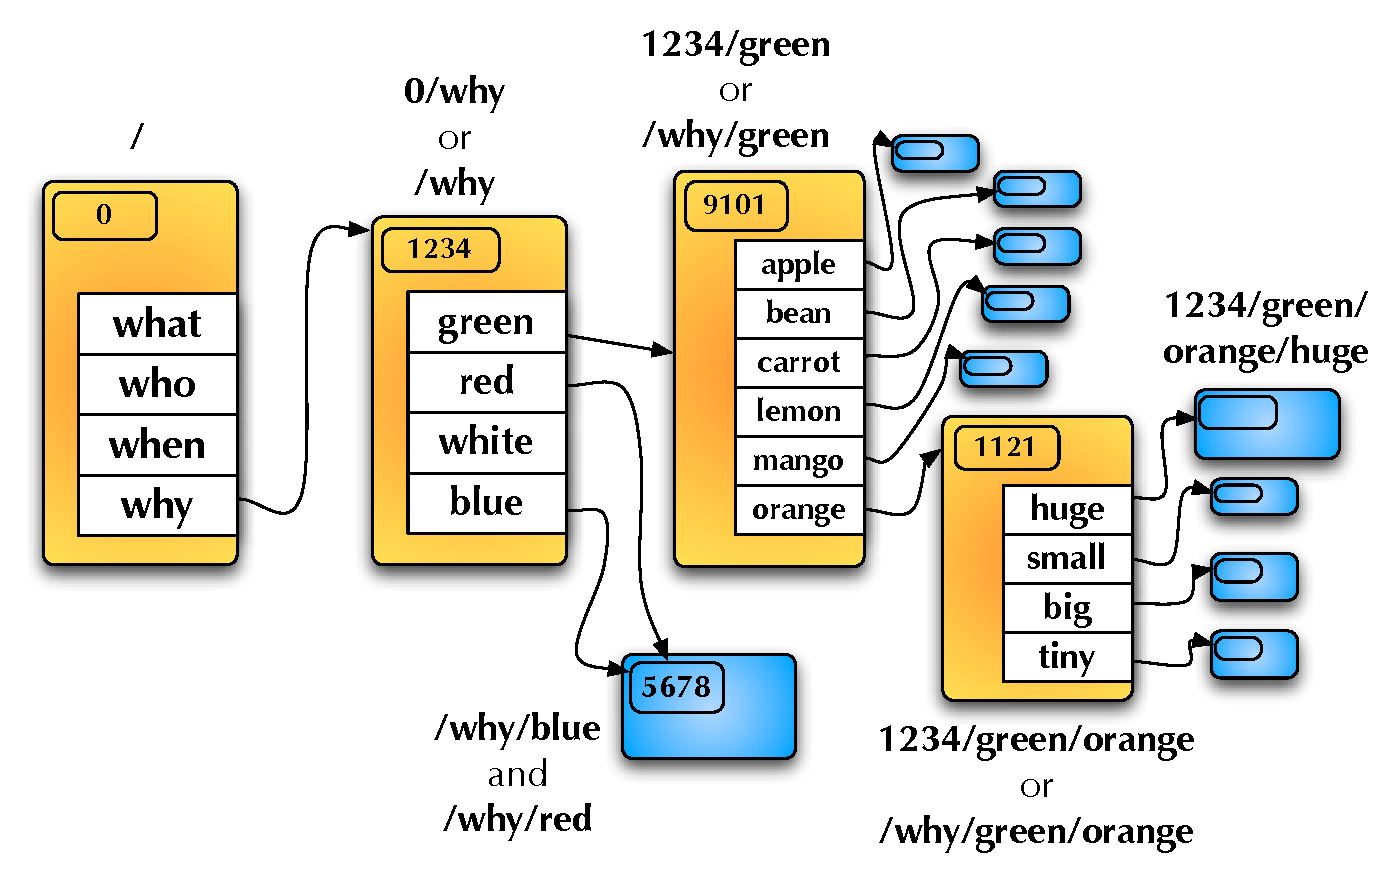
\includegraphics{arc-storage-namespace.pdf}}}
\caption{\label{fig:namespace}Example of the hierarchy of the global namespace} }
\end{figure}

Example on Figure~\ref{fig:namespace}: if we have a collection with GUID \verb#1234#, and there is a collection called \verb#green# in it, and in \verb#green# there is another collection called \verb#orange#, and in \verb#orange# there is a file called \verb#huge#, then we can refer to this file with the Logical Name \verb#1234/green/orange/huge#, which means that from the collection called \verb!1234! we have to follow along the path: \verb!green!, \verb!orange!, \verb!huge!.

There is a dedicated root collection (which has the GUID \verb#0#), and if a LN starts with no GUID prefix, it is implicitly prefixed with the GUID of this well-known root collection, e.g.~\verb#/why/blue# means \verb#0/why/blue#. If a user wants to find the file called \verb#/why/blue#, the system knows where to start the search: the GUID of the root collection. The root collection knows the GUID of \verb#why#, and the (sub-)collection \verb#why# knows the GUID of \verb#blue#. If the GUID of this file is \verb#5678#, and somebody makes another entry in collection \verb#/why# (= \verb#0/why#) with name \verb#red# and GUID \verb#5678#, then the \verb#/why/red# LN points to the same file as \verb#/why/blue#, which concept is very similar to a hardlink in a regular local file system.

% section files_and_collections (end)

\section{Storage nodes and replicas} % (fold)
\label{sec:storage_nodes_and_replicas}

The collections in the ARC storage are logical entities, the content of a collection is stored as metadata of the collection, which means the a collection actually has no physical data. A file however has both metadata and real physicial data (the actual bytes of the file). The metadata of a file is stored in the same database where the collections are stored, but the physical data of a file is stored on storage nodes as multiple replicated copies.

A storage node consists of two things: a storage element service which is capable of storing and serving files through a specific protocol (e.g. a web server, an FTP server, a GridFTP server, etc.) and a Shepherd service which provides a simple interface to access the storage node, and which can initiate and manage file transfers through the storage element service. The Shepherd has different backends for the supported storage element services which made it possible the communicate with them.

So we have logical files, which are part of the hierarchical namespace and have a GUID and other metadata, and a logical file has one or more physical replicas. The physical replicas stored on seperate storage nodes. In order to connect the logical file to its replicas, we need to have some pointers. Each storage node has a URL and each replica has a unique ID within the storage node called \emph{referenceID}, the URL and the referenceID together is called a \emph{Location}, a Location unambiguously points to one specific replica. So to connect the logical files to the physical ones, each logical file has a list of Locations.



%%%%%%%%%%%%%%%%%%%%%%%%%%%%%%%%%%%%%%



% section storage_nodes_and_replicas (end)

\section{The Bartenders} % (fold)
\label{sec:the_bartenders}

The Bartender service provides a high-level interface for the storage system to the clients. You can create and remove collections, create, get and remove files, move files and collections within the namespace using Logical Names. The Bartender communicates with the Librarian and Shepherd services to accomplish the client’s requests. The actual file data does not go through the Bartender; file transfers are directly performed between the storage nodes and the clients. There could be any number of independent Bartender services in the system which provides high-availability and load-balancing.

% section the_bartenders (end)

\section{The Librarians} % (fold)
\label{sec:the_librarians}
The Librarian is capable of managing the hierarchy and metadata of files and collections, and health information of the Shepherd services. Each file and collection in the Librarian has a globally unique ID (GUID). A collection contains files and other collections, and each of these entries has a name unique within the collection very much like entries in a usual directory on a local filesystem. Besides files and collections the Librarian stores a third type of entries called Mount Points which are references to external services which will be in the future used to mount the namespace of third-party storages to our global namespace and make the files on a third-party storage available through the interface of the ARC storage system.

The Librarian also manages information about registered Shepherd services which are associated with a storage node, and receives heartbeat messages from them and change replica states automatically if needed.

The Librarian uses the A-Hash as database, that’s why there could be any number of independent Librarian services (all using the same A-Hash) which provides high-availability and load-balancing.

% section the_librarians (end)

\section{The A-Hash} % (fold)
\label{sec:the_a_hash}
The A-Hash is a currently centralized, but later distributed service capable of consistently storing objects containing property-value pairs organized in sections. All metadata about files and collections are stored in the A-Hash, and some information about Shepherd services is stored in it as well. The A-Hash itself does not interpret the data, it just stores tuples of strings.

% section the_a_hash (end)

\section{The Shepherds} % (fold)
\label{sec:the_shepherds}
When a new file is put into the system the number of needed replicas is given for the file. The file replicas are stored on different storage nodes, for each storage node there is Shepherd service which manages the storage node, reports its health state to the Librarian and provides the interface for initiating file transfer.

The file-naming used by a Shepherd has nothing to do with the the hierarchy of collections, or Logical Names. When a new replica upload is initiated, the Shepherd generates an ID which refers to it within that Shepherd. Each Shepherd has a unique ID itself, so with these IDs the replica can be unambiguously referenced, this is called a \emph{Location}. The namespace of these Locations has nothing to do with the namespace of GUIDs or the namespace of Logical Names. It consists of two IDs: the ID of the Shepherd and the ID of the file within the Shepherd: \verb!(serviceID, referenceID)!

% section the_shepherds (end)

\section{Heartbeats and replication} % (fold)
\label{sec:heartbeats_and_replication}
Each Shepherd should periodically send heartbeats to a Librarian service with information about replicas whose state changed since the last heartbeat, the Librarian stores these file lists (which contains the GUIDs of the files as well), and if it doesn’t receive a heartbeat for a Shepherd in a given time, it invalidates all the replicas the Shepherd stores. This invalidating means that the state of that location will be \verb!offline!.

If a Shepherd finds out that a file is missing or has a bad checksum, it reports that the file is \verb#invalid# to the Librarian immediately, and the Librarian alters the state of the given replica of the file. The Shepherd tries to recover its replica by downloading it from another Shepherd. In order to do this the Shepherd contacts a Bartender and asks for the file. The Bartender chooses a valid replica, initiate file transfer by a Shepherd having a valid replica, and returns the TURL to the Shepherd with the invalid replica. The Shepherd with the invalid replica downloads the file from the other Shepherd, and if everything is OK, signals to the Librarian that the replica is \verb!alive! again.

The Shepherds periodically ask the Librarian whether the files they store have enough replicas. If a Shepherd finds that one of the files has not enough replica it turns to a Bartender offering replication. The Bartender chooses a Shepherd, initiates a put request then returns the TURL to the offering Shepherd which could upload the replica. The Shepherd who now has the new replica notifies the Librarian that the file is \verb!alive!. The Librarian sets the state of this new replica.

% section heartbeats_and_replication (end)

\section{Security} % (fold)
\label{sec:security}

The current version of the ARC storage system has no implemented solution for security issues. Designing and implementing a powerful, flexible, fine-grained solution for authentication and authorization is very important. Currently we have plans how to do that, and the design of the storage services makes it easy to integrate the chosen solution into the system.

For additional details, see Section~\ref{sec:plans_for_security}.

% section security (end)


\chapter{Use cases} % (fold)
\label{cha:use_cases}

\section{Downloading a file} % (fold)
\label{sec:downloading_a_file}
\begin{figure}[ht]
\centering{{\scalebox{0.7}{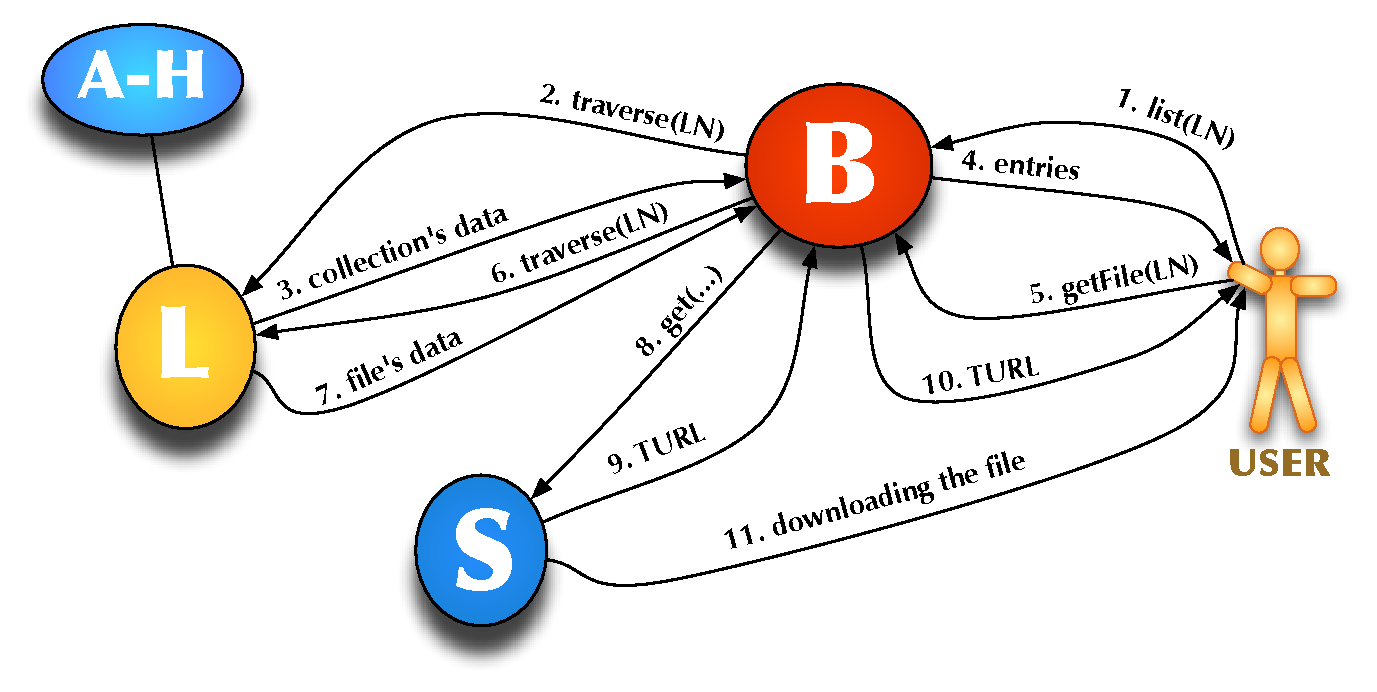
\includegraphics{arc-storage-downloading.pdf}}}
\caption{\label{fig:downloading}Downloading a file} }
\end{figure}

We want to download a file about which we know that it is somewhere in our home collection on the storage (see Figure~\ref{fig:downloading}). The LN of our home collection is e.g.~\verb#/ourvo/users/we# (here a `home collection' could be just a collection which is given to us by our VO). We can get a list of entries in this collection from any Bartender.

\begin{enumerate}
\item We need to find a Bartender. Maybe we have a cached list of recently used Bartenders or we can get one from the information system. When we have an endpoint reference of a Bartender, we could call its list method with the LN \verb#/ourvo/users/we#.
\item The Bartender has to find a Librarian service, again using its cache of recently used Librarian services or get a new one from the information system. When the Bartender has an endpoint reference of a Librarian service, it could ask the Librarian to traverse the LN \verb#/ourvo/users/we#.
\item The Librarian needs the A-Hash service to access the stored data, when it has the endpoint reference of the A-Hash service, it could get the information about the root collection, which contains the GUID of the \verb#ourvo# sub-collection. Then the Librarian gets the entries of this \verb#ourvo# collection, and in it it can find the GUID of \verb#users#, and in the entries of \verb#users# there is the GUID of \verb#we#, which the Librarian returns to the Bartender with all the metadata.
\item The Bartender now has the GUID and the metadata of the collection \verb#/ourvo/users/we#, including the list of its entries. This is returned to us.
\item So we get the list of our \verb#/ourvo/users/we# collection, and now we realize that the file we want has the LN \verb#/ourvo/users/we/thefilewewant# and we know the GUID of it as well: e.g.~\verb#a4b2e#. (Of course we know the GUID of the \verb#/ourvo/users/we# collection too, which is e.g.~\verb#13245# and using this we could refer to our file as \verb#13245/thefilewewant# which means the entry called \verb#thefilewewant# in the collection with a GUID \verb#13245#.) We connect a Bartender again (the same one or maybe another one) to get the file with any of these LNs, the \verb#a4b2e# is the fastest solution because the Bartender need not to look up the whole LN again in the Librarian, a well-written client API should use this. With the get request we give the Bartender the list of transfer protocols we are able to use.
\item The Bartender contacts the Librarian to get the locations of the replicas of this file.
\item The Librarian returns all the metadata of the requested LN.
\item The Bartender chooses a `location' which consists of the ID of a Shepherd, and the referenceID of the file within the Shepherd. Using the information system or its local cache it could get the endpoint reference of the Shepherd. The Bartender initiates a transfer by the Shepherd, if the Shepherd supports one of the transfer protocols we give, it can create a transfer URL (TURL) with a protocol we can download.
\item The Shepherd returns the TURL to the Bartender.
\item The Bartender returns the TURL to us.
\item Now we have a TURL from which we can download it.
\end{enumerate}

% section downloading_a_file (end)

\section{Uploading a file} % (fold)
\label{sec:uploading_a_file}

\begin{figure}[ht]
\centering{{\scalebox{0.7}{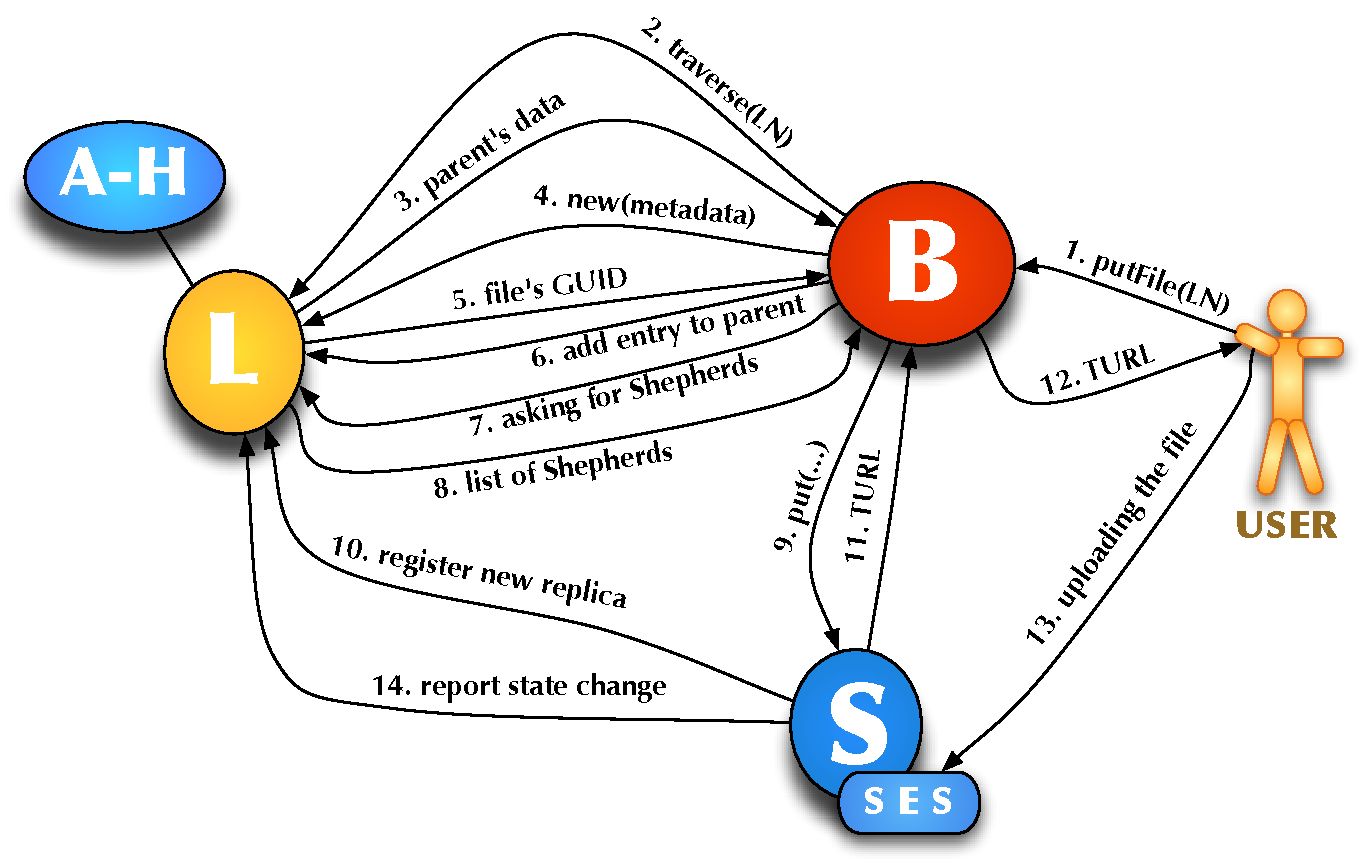
\includegraphics{arc-storage-uploading.pdf}}}
\caption{\label{fig:uploading}Uploading a file} }
\end{figure}

We have a file on our local disk we want to upload to a collection called \verb#/ourvo/common/docs#. (See Figure~\ref{fig:uploading}.)
\begin{enumerate}
\item We contact a Bartender to put the file, we give the size and checksum and other metadata, and the transfer protocols we want to use. And of course we give the Logical Name we want to be the name of the file, which in this case will be \verb#/ourvo/common/docs/proposal.pdf#
\item The Bartender ask a Librarian to traverse this LN.
\item If the Librarian can traverse the whole LN then this LN is already exists, but if the LN is still available and the parent exists, the Librarian’s response contains the GUID and metadata of the parent collection.
\item Then the Bartender creates a new file entry within the Librarian with all the information we gave. 
\item The Librarian returns the GUID of this new entry.
\item Then the Bartender add the name \verb#proposal.pdf# and the new GUID to the collection \verb#/ourvo/common/docs# and from now on there will be a valid LN \verb#/ourvo/common/docs/proposal.pdf# which points to a file which has no replica at all. If someone tried to download the file called \verb#/ourvo/common/docs/proposal.pdf# now, would get an error message `try again later'.
\item The Bartender (using the information system) chooses a Shepherd and gets its endpoint reference. Then the Bartender initiates uploading of the file to the Shepherd: the request includes the size and checksum of the file, the GUID, and the protocols we are able to use.
\item The Shepherd creates a transfer URL and a referenceID for this file and registers the GUID of the file in its own database and reports to the Librarian that there is a new replica with state \verb#creating#. The Librarian gets the message from the Shepherd and creates a new entry in the locations list of the given file with the serviceID and the referenceID the Shepherd have just reported. If someone tries to download this file now, still gets a `try again later' error message, because this new replica is still not \verb#alive#.
\item The Shepherd returns the the TURL to the Bartender.
\item The Bartender returns the TURL to us.
\item Then we can upload the file to this TURL.
\item The Shepherd detects that the file is arrived and reports the change of state to \verb#alive# to the  Librarian who alters the state in the given file-entry. At this point the file has only one replica. 
\end{enumerate}
\begin{itemize}
\item The Shepherd periodically checks the Librarian if this is less than the needed replica number, and if it is then it initiates creating a new replica by a Bartender.
\item The Bartender chooses another Shepherd, initiates the transfer then returns the TURL to the  first Shepherd which uploads the file to the new Shepherd.
\item All the Shepherds check periodically whether their files have enough replica, and if any of them find that there is more replica needed, it initiates creating a new. If more than one Shepherd of course could cause that there will be more replicas than needed. If a Shepherd finds out that a file has more replicas than needed it notifies a Bartender about it.
\item The Bartender ask the Librarian about all Shepherds this file has replicas on, flags this file as `removing a replica' which prevents other Bartenders to remove an other replica accidentally, then make a decision of which one is to be removed, then contacts the chosen Shepherd and asks it to remove the replica. The Shepherd then notify the Librarian, and the Librarian removes the replica, and removes the flag `removing a replica' as well.
\item If the client cannot upload the file to the given TURL for some reason, it is possible to call \verb#addReplica# to get a new TURL without removing and recreating the file.
\end{itemize}

% section uploading_a_file (end)

\section{Removing a file} % (fold)
\label{sec:removing_a_file}

\begin{figure}[ht]
\centering{{\scalebox{0.7}{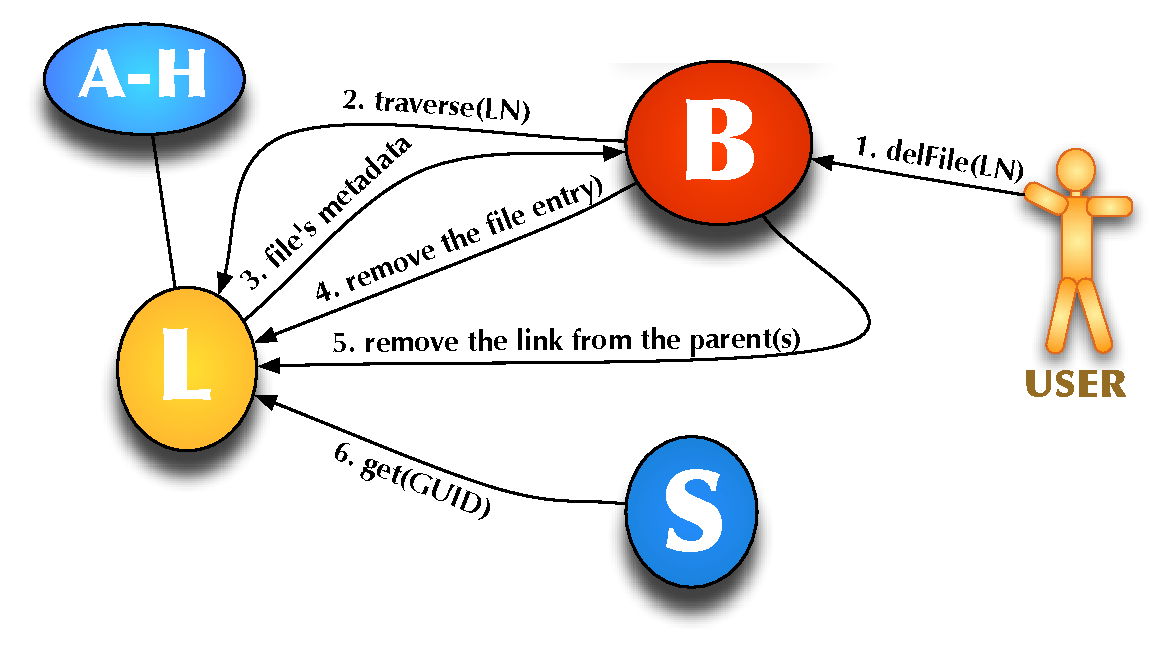
\includegraphics{arc-storage-removing.pdf}}}
\caption{\label{fig:removing}Removing a file} }
\end{figure}
\begin{enumerate}
    \item If we want to remove a file, we should connect to a Bartender with the LN of the file we want to remove.
    \item The Bartender asks the Librarian to traverse the LN and return the list of parent collections of this file.
    \item The Librarian returns the data.
    \item If the file has only parent, it asks the Librarian to remove the file entry itself, and the entry from the parent collection. If the file has more parent collections (hard links) the Bartender only removes the entry from the parent collection and removes the parent from the list of parent  collections of this file.
    \item Next time the Shepherd does its periodic check, it asks the Librarian about each of its stored replicas, and finds out that one of them no longer exists, so it removes the replica from the storage node.
\end{enumerate}


% section removing_a_file (end)

% chapter use_cases (end)

\chapter{Technical description and implementation status} % (fold)
\label{cha:technical_description_and_implementation_status}

The services are written in Python and running in the HED\footnote{The ARC container - \url{https://www.knowarc.eu/documents/Knowarc\_D1.2-2\_07.pdf}} hosting environment. The HED itself is written in C++, but there are language bindings which allow us to write services in other languages, e.g.~in Python or Java. The source code of the storage services are in the NorduGrid Subversion repository\footnote{\url{http://svn.nordugrid.org/trac/nordugrid/browser/arc1/trunk/src/services/storage}}.

The current version of the prototype has no information system and no security, these are soon to be integrated to the system.

The information system is needed to discover services, and to translate \emph{serviceID}s to endpoint references (URLs). Currently the URLs are written in the configuration files, and the Shepherd services are reporting their URLs to the Librarian, so the Bartender could ask for all alive Shepherds.

Some self-healing mechanisms are not implemented yet, e.g. the files and collections contains their parent-collections as their metadata, and of course a collection contains a list of its files and sub-collections, and if somehow this information became inconsistent, the system should detect and repair it. This is not implemented yet.

\section{Plans for security} % (fold)
\label{sec:plans_for_security}

Security is needed to do proper authorization of the users, and to manage access policies of files and collections. ARC has its own policy language, for each file and collection there will be a policy XML document stored as a metadata. The storage services will use these policies and the properties extracted from the communication channel to make authorization decisions. If the properties and the policies are present, the decision will be actually made by the security framework of HED.

These are the planned actions which can be used for access control:
\begin{itemize}
    \item \emph{read}: user can get the list of entries in the collection; user can download the file
    \item \emph{addEntry}: user can add a new entry to the collection;
    \item \emph{removeEntry}: user can remove any entry from the collection 
    \item \emph{delete}: user can delete the collection if it is empty; user can delete a file (if you want to remove a file/collection, then the Bartender needs to remove the entry from the parent collection, and then delete the file/collection itself, so you need to have both permissions)
    \item \emph{modifyPolicy}: user can modify the policy of the file/collection
    \item \emph{modifyStates}: user can modify some special metadata of the file/collection (close the collection, change the number of needed replica of the file)
    \item \emph{modifyMetadata}: user can modify the arbitrary metadata section of the file/collection (these are key-value pairs)
\end{itemize}
When a user has the permission in the Librarian to download a file then the user should have permission to access at least one of the file's replica, so there should be a Shepherd which allows the user the get the file. If the Bartender has permission to access the Shepherd, then the Bartender should create an assertion which allows the user to access the file. This could be a signed token which contain a policy defining access to particular file. But all these are currently just plans.

% section plans_for_security (end)

Further prototype statuses and plans can be found below within each section about the services.

% chapter technical_description_and_implementation_status (end)
\newpage

\section{A-Hash} % (fold)
\label{sec:a_hash}

\subsection{Functionality} % (fold)

The A-Hash will be a distributed service capable of storing tuples of strings in a scalable manner. Currently it only has a centralized implementation. It stores \emph{objects}, where each object has an arbitrary string \emph{ID}, and contains any number of \emph{property}-\emph{value} pairs grouped in \emph{section}s, where \emph{property}, \emph{value} and \emph{section} are arbitrary strings. There could only be a single \emph{value} for a \emph{property} in a \emph{section}.

If you have an ID, you can get all property-value pairs of the corresponding object with the \emph{get} method, or you could specify only which sections or properties do you need. You can add or remove property-value pairs of an object or delete all occurrences of a property or create a new object with the \emph{change} method, and you can specify conditions, which means the change is only applied if the given conditions are met.

% subsection functionality (end)

\subsection{Prototype status and plans} % (fold)

The A-Hash service currently implemented as a single central service, which stores the data on disk in separate files per \emph{object}. Fall of 2008 it will be reimplemented using a distributed hash table (DHT) algorithm, one possible candidate is the Chord\footnote{The Chord project - \url{http://pdos.csail.mit.edu/chord/}} algorithm with a consistency solution called Etna\footnote{Etna: a Fault-tolerant Algorithm for Atomic Mutable DHT Data - \url{http://pdos.csail.mit.edu/\~athicha/papers/etna.ps}} on top of it. This reimplementation hopefully won’t change the interface of the service.

% subsection prototype_status_and_plans (end)

\subsection{Data model} % (fold)

\begin{itemize}
    \item \emph{ID} is an arbitrary string
    \item \emph{object} contains property-value pairs in sections, technically it is a list of key-\emph{value} pairs where the key is a (\emph{section}, \emph{property}) tuple
\end{itemize}

% subsection data_model (end)

\subsection{Interface} % (fold)

\begin{description}
    \item [get(ids, neededMetadata)] returns \emph{getResponse} which is a list of (\emph{ID}, \emph{object}) pairs.

    The \emph{ids} is a list of string \emph{ID}s, \emph{neededMetadata} is a list of (\emph{section}, \emph{property}) pairs. For each \emph{ID} it returns all the \emph{value}s for each \emph{property} in each \emph{section} (filtered by \emph{neededMetadata}), so \emph{object} is a list of (\emph{section}, \emph{property}, \emph{value}) tuples.

    \item [change(changeRequest)] returns \emph{changeResponse} which is a list of (\emph{changeID}, \emph{success}, \emph{failedConditionID}) tuples.

    \emph{changeRequest} is a tuple of (\emph{changeID}, \emph{ID}, \emph{changeType}, \emph{section}, \emph{property}, \emph{value}, \emph{conditions}), where \emph{changeID} is an arbitrary ID to identify in the response which change was successful; \emph{ID} points to the object we want to change; \emph{changeType} can be `\textbf{set}' (set the property within the section to value), `\textbf{unset}' (remove the property from the section regardless of the value), `\textbf{delete}' (removes the whole object), conditions is a list of (\emph{conditionID}, \emph{type}, \emph{section}, \emph{property}, \emph{value}) tuples, where \emph{type} could be `\textbf{is}' (the property in the section is set to the value), `\textbf{isnot}' (the property in the section is not set to the value), `\textbf{isset}' (the property of the section is set to any value), `\textbf{unset}' (the property of the section is not set at all).
    If all conditions are met, tries to apply changes to the objects, creates a new object if a previously non-existent ID is given. If one of the conditions is not met, returns the ID of the failed condition.
\end{description}
    
% subsection interface (end)

% section a_hash (end)
\newpage

\section{Librarians} % (fold)
\label{sec:librarian}

\subsection{Functionality} % (fold)
% 
The Librarian manages a tree-hierarchy of files, grouping them into collections. There is a root collection with a well-known GUID which can be used as starting point when resolving Logical Names. If you create a new collection with the method \emph{new}, the Librarian generates a new GUID, but does not insert it into the tree-hierarchy which can be done by adding this GUID as a new entry to one of the existing collection using the \emph{modifyMetadata} method of the existing collection which makes it the parent of the new collection. A collection can be closed via metadata modification which cannot be undone and prevents files to be added or removed from this collection. A new file  also can be created with the \emph{new} method which returns the newly generated GUID of the new file entry which should be added to a parent collection to insert it into the global namespace. A file has a list of locations where its replicas are stored, this list too can be manipulated with \emph{modifyMetadata}. The access policies of the files and collections are also stored as metadata. The \emph{remove} method deletes an entry from the Librarian. The \emph{traverseLN} method try to traverse Logical Names by walking the hierarchy of the namespace and to return the GUID of the entry pointed by the LN. After you have a GUID of file, collection or mount point, you can get all the information using the \emph{get} method. 

% subsection functionality (end)

\subsection{Prototype status and plans} % (fold)

The Librarian service currently implements all the methods below, but doesn't do very much error checking. This should be changed, the Librarian should check the validity of metadata, and forbid some cases, e.g.~reopen a closed collection.

% subsection prototype_status_and_plans (end)

\subsection{Data model} % (fold)
\label{sub:data_model}
Each librarian entry has a unique ID called \emph{GUID}.

The Librarian uses the A-Hash to store all the data about files and collections. The A-Hash is capable of storing property-value pairs organized in sections, which actually means that it stores (\emph{section}, \emph{property}, \emph{value}) tuples where each member is simply a string, e.g.~(`entry', `type', `collection') or (`ACL', `johnsmith', `owner') or (`timestamps', `created', `1196265901') or (`locations', `64CDF45F-DDFA-4C1D-8D08-BCF7810CB2AB:9A293F27DC86', `sentenced'). There could be only one \emph{value} for a (\emph{section}, \emph{property}) pair.

\begin{itemize}
    \item A \textbf{collection} is a list of files and other collections, which are in parent-children relationships forming a tree-hierarchy. Each entry has a name which is only valid within this collection, and it is unique within the collection. Each entry is referenced by its GUID. So the metadata sections of a collection are as follows: 
    \begin{description}
        \item [entry] section 
        \begin{itemize}
            \item \emph{type}: `collection' 
        \end{itemize}
        \item [entries] section 
        \begin{itemize}
            \item \emph{(name, GUID) pairs}: a Collection is basically a list of name-GUID pairs. 
        \end{itemize}
        \item [timestamps] section 
        \begin{itemize}
            \item \emph{created}: timestamp of creation 
            \item \emph{modified}: timestamp of last modification 
        \end{itemize}
        \item [states] section 
        \begin{itemize}
            \item \emph{closed}: if the collection is closed, then nothing can be added to its contents 
        \end{itemize}
        \item [policies] section 
        \begin{itemize}
            \item XML representations of access policies 
        \end{itemize}
        \item [metadata] section 
        \begin{itemize}
            \item any other arbitrary metadata 
        \end{itemize}
    \end{description}
    \item A \textbf{file} entry contains the following sections: 
    \begin{description}
        \item [entry] section 
        \begin{itemize}
            \item \emph{type}: `file' 
        \end{itemize}
        \item [locations] section 
        \begin{itemize}
            \item \emph{(location, state) pairs}, where a location is a (\emph{serviceID}, \emph{referenceID}) pair serialized as a  string, where \emph{serviceID} is the ID of the Shepherd service storing this replica, \emph{referenceID} is the ID of the file within that Shepherd service, and state could be `\textbf{alive}' (if the replica passed the checksum test, and the Shepherd reports that the storage node is healthy), `\textbf{invalid}' (if the replica has wrong checksum, or the Shepherd claims it has no such file), `\textbf{offline}' (if the Shepherd is not reachable, but may have a valid replica), `\textbf{creating}' (if the replica is in the state of uploading), `\textbf{sentenced}' (if the replica is marked for deletion) 
        \end{itemize}
        \item [timestamps] section 
        \begin{itemize}
            \item \emph{created}: timestamp of creation 
            \item \emph{modified}: timestamp of last modification (e.g.~modification of metadata)
        \end{itemize}
        \item [states] section 
        \begin{itemize}
            \item \emph{size}: the file size in bytes
            \item \emph{checksum}: checksum of the file
            \item \emph{checksumType}: the name of the checksum method
            \item \emph{neededReplicas}: how many valid replicas should this file have 
        \end{itemize}
        \item [policies] section 
        \begin{itemize}
            \item XML representations of access policies 
        \end{itemize}
        \item [metadata] section 
        \begin{itemize}
            \item any other arbitrary metadata 
        \end{itemize}
    \end{description}
    \item There is one more type of Librarian entries called \textbf{mount point} which is a reference to a service which is capable of handling a subtree of the namespace. The properties of a mount point in sections:
    \begin{description}
        \item [entry] section 
        \begin{itemize}
            \item \emph{type}: `mountpoint' 
        \end{itemize}
        \item [mount] section 
        \begin{itemize}
            \item \emph{target}: the ID of the service
            \item \emph{ID}: an ID within the service (optional)
        \end{itemize}
        \item [timestamps] section 
        \begin{itemize}
            \item \emph{created}: timestamp of creation 
            \item \emph{modified}: timestamp of last modification (e.g.~modification of metadata)
        \end{itemize}
        \item [policies] section 
        \begin{itemize}
            \item XML representations of access policies 
        \end{itemize}
        \item [metadata] section 
        \begin{itemize}
            \item any other arbitrary metadata 
        \end{itemize}
    \end{description}

    \item The Librarian stores information about the Shepherds, so each Shepherd has a GUID as well. There is an entry (with GUID `1' by default) which contains the GUID and the timestamp of the last heartbeat for each registered Shepherd:
    \begin{description}
    	\item [nextHeartBeat] section
    	\begin{itemize}
    		\item (ID, timestamp) pairs
    	\end{itemize}
    	\item [serviceGUID] section
        \begin{itemize}
            \item (ID, GUID) pairs
        \end{itemize}
    \end{description}

    \item For each Shepherd there is a separate entry with the list of files:
    \begin{description}
    	\item [entry] section
        \begin{itemize}
            \item \emph{type}: `shepherd'
        \end{itemize}
    	\item [files] section
    	\begin{itemize}
    	    \item \emph{(referenceID, GUID) pairs} for each replica stored on the Shepherd
    	\end{itemize}
    \end{description}
\end{itemize}

% subsection data_model (end)

\subsection{Interface} % (fold)

 \begin{description}
    \item[new(newRequestList)] returns a list of (\emph{requestID}, \emph{GUID}, \emph{success})
    
    \emph{newRequestList} is a list of (\emph{requestID}, \emph{metadata}) where \emph{requestID} is an arbitrary ID used to identify this request in the list of responses; \emph{metadata} is a list of (\emph{section}, \emph{property}, \emph{value}) tuples.
    This method generates a \emph{GUID} for each request, and inserts the new entry (with the given metadata) into the A-Hash, then returns the GUIDs of the newly created entries. The (`entry', `type') property of the metadata contains whether it is a file or a collection.
    
    \item[modifyMetadata(modifyMetadataRequestList)] returns a list of (\emph{changeID}, \emph{success})

    \emph{modifyMetadataRequestList} is a list of (\emph{changeID}, \emph{GUID}, \emph{changeType}, \emph{section}, \emph{property}, \emph{value}) where \emph{changeType} can be `\textbf{set}' (set the property in the section to value), `\textbf{unset}' (remove the property-value pair from the section), `\textbf{add}' (set the property in the section to value only if it is not exists already).
    
    \item [get(GUIDs, neededMetadata)] returns \emph{getResponse}
    
    \emph{GUIDs} is a list of GUIDs, \emph{neededMetadata} is a list of (\emph{section}, \emph{property}) pairs indicating only which properties we need, \emph{getResponse} is a list of (\emph{GUID}, \emph{metadata}) where metadata is a list of (\emph{section}, \emph{property}, \emph{value}) tuples. This method returns the metadata of all the \emph{GUID}s filtered with \emph{neededMetadata}.
    
    \item [remove(removeRequestList)] returns a list of (\emph{requestID}, \emph{success}) pairs
    
    \emph{removeRequestList} is a list of (\emph{requestID}, \emph{GUID}) pairs. \emph{success} could be `\textbf{removed}' or `\textbf{failed}: reason'.
    
    \item [traverseLN(traverseRequestList)] returns \emph{traverseResponseList}
    
    \emph{traverseRequestList} is a list of (\emph{requestID}, \emph{LN}) with the Logical Names to be traversed
    
    \emph{traverseResponseList} is a list of (\emph{requestID}, \emph{metadata}, \emph{GUID}, \emph{traversedLN}, \emph{restLN}, \emph{wasComplete}, \emph{traversedList}) where:
    \begin{description}
        \item[metadata] is all the metadata of the of traversedLN in the form of (\emph{section}, \emph{property}, \emph{value}) tuples
        \item[GUID] is the \emph{GUID} of the \emph{traversedLN}
        \item[traversedLN] is the part of the \emph{LN} which was traversed, if \emph{wasComplete} is true, this should be the full \emph{LN}
        \item[restLN] is the postfix of the \emph{LN} which was not traversed for some reason, if \emph{wasComplete} is true, this should be an empty string
        \item[wasComplete] indicates whether the full \emph{LN} was traversed
        \item[traversedList] is a list of (\emph{LNpart}, \emph{GUID}) pairs, where \emph{LNpart} is a part of the \emph{LN}, \emph{GUID} is the GUID of the Librarian-entry referenced by that part of the \emph{LN}, the first element of this list is the shortest prefix of the \emph{LN}, the last element is the \emph{LN} without its last part
    \end{description}
    
    \item [report(serviceID, filelist)] returns in \emph{nextReportTime} a number of seconds, which is the timeframe within the Librarian expects the next heartbeat from the Shepherd
    
    \emph{filelist} is a list of (\emph{GUID}, \emph{referenceID}, \emph{state}) tuples containing the state of changed or new files, where \emph{state} could be `\textbf{invalid}' (if the periodic self-check of the Shepherd found a non-matching checksum or missing file), `\textbf{creating}' (if this is a new file not uploaded yet) or `\textbf{alive}' (if the file is uploaded and the checksum is OK).
    
\end{description}


% subsection interface (end)

% section librarian (end)
\newpage

\section{Shepherds} % (fold)
\label{sec:shepherds}

\subsection{Functionality} % (fold)

A Shepherd service is capable of managing a storage node. It keeps track all the files it stores with their GUIDs and checksums. It periodically checks each file to detect corruption, and send reports to a Librarian indicating that the storage node is up and running, and whether some file's state has been changed. If a file goes missing or has a bad checksum then the Librarian is notified about the error (here the Shepherd refers to the file with its GUID, that's why it needs to store the GUIDs of its files). It periodically asks the Librarian how many replicas its files have, and if a file has fewer replicas than needed, the Shepherd offers its copy for replication by calling the Bartender.

A Shepherd service is always connected to a file transfer service (e.g.~`HTTP(S)', `FTP(S)', `ByteIO', `GridFTP', etc.). For each supported file transfer service we need a backend module which makes the Shepherd capable of communicating with the file transfer service to initiate file transfers, to detect whether a transfer was successful or not, to generate local IDs and checksums, etc.

A file in a storage node could be identified with a \emph{referenceID} which is unique within that node. If we know the \emph{location} of a file, which is the ID of the Shepherd service (\emph{serviceID}) and the \emph{referenceID}, we could get the endpoint reference (URL) of the Shepherd from the information system, then we could call its \emph{get} method with the \emph{referenceID} and a list of transfer protocols we can use (e.g.~`HTTP', `FTP'), the Shepherd chooses a protocol from this list which it can provide, and create a transfer URL (\emph{TURL}) and returns it along with the \emph{checksum} of the file. We could download the file from this \emph{TURL}, and verify it with the \emph{checksum}. An end user of the storage system does not need to call this \emph{get} method, because the Bartender service will do it, the user just asks the Bartender and gets the TURL.

Storing a file starts with initiating the transfer with the \emph{put} method of the Shepherd, we should give the \emph{size} and \emph{checksum} of the file and its \emph{GUID} as well. We also specify a list of transfer protocols we are able to use, and the Shepherd chooses a \emph{protocol}, creates a \emph{TURL} for uploading and generates a \emph{referenceID}, then we can upload the file to the TURL. Again, the end user just asks the Bartender, and gets the TURL, the user does not need to call the \emph{put} method of the Shepherd directly.

These \emph{TURL}s are one-time URLs which means that after the client uploads or downloads the file these \emph{TURL}s cannot be used again to do the same. If we want to download the same file twice, we have to initiate the transfer twice, and will get two different \emph{TURL}s.

With the \emph{stat} method we can get some information about a replica, e.g.~checksum, GUID, state (`creating', `alive' or `invalid'), etc. The \emph{delete} method removes the file.

In normal operation the \emph{put} and \emph{get} calls is made by a Bartender but the actual uploading and downloading is done by the user's client. In the case of replication a Shepherd with a valid replica initiates the replication, this Shepherd asks the Bartender to choose a new Shepherd, the Bartender initiates putting the new replica on a chosen Shepherd and receives the TURL, then the Bartender returns the TURL to the initiator Shepherd, which uploads its replica to the given TURL.

% subsection functionality (end)

\subsection{Prototype status and plans} % (fold)

The current implementation of the Shepherd service has a working \emph{get}, \emph{put}, \emph{stat}, \emph{delete} methods, and a method called \emph{toggleReport} which can be used the simulate storage node failure with the Shepherd not reporting to a Librarian. 
There is a separate service which provide a subset of the ByteIO interface, and there is an other separate service which is a basic HTTP server, these are both could be used as file transfer services, both have its backend module for the Shepherd. Currently both file transfer services have the problem of using too much memory while transferring files.
Further plans include better file transfer services and backend modules for third-party file transfer services.

% subsection prototype_status_and_plans (end)

\subsection{Data model} % (fold)

A file of a Shepherd service is referenced by its \emph{referenceID}. Each file has a \emph{state} which could be `\textbf{creating}' when the transfer is initiated but the file is not uploaded yet, `\textbf{alive}' if the file is uploaded and has a proper checksum, or `\textbf{invalid}' if it does not exists anymore or has a bad checksum. Each file has a \emph{localID} which is used in the backend modules.

% subsection data_model (end)



\subsection{Interface} % (fold)

\begin{description}
    \item[get(getRequestList)] returns list of (\emph{requestID}, \emph{getResponseData})
    
    \emph{getRequestList} is a list of (\emph{requestID}, \emph{getRequestData}) where \emph{requestID} is an arbitrary ID used in the reply
    
    \emph{getRequestData} is a list of (\emph{property}, \emph{value}) pairs, where mandatory properties are: `\textbf{referenceID}' which refers to the file to get and `\textbf{protocol}' indicates a protocol the client can use (there could be multiple protocols in getRequestData).
    
    \emph{getResponseData} is a list of (\emph{property}, \emph{value}) pairs, such as: `\textbf{TURL}' is a transfer URL which can be used by the client to download the file; `\textbf{protocol}' is the protocol of the TURL; `\textbf{checksum}' is the checksum of the replica; `\textbf{checksumType}' is the name of the checksum method and `\textbf{error}' could contain an error message if there is one.
     
    \item[put(putRequestList)] returns a list of (\emph{requestID}, \emph{putResponseData})
    
    \emph{putRequestList} is a list of (\emph{requestID}, \emph{putRequestData}) where \emph{requestID} is an ID used for the response
    
    \emph{putRequestData} is a list of (\emph{property}, \emph{value}) pairs such as `\textbf{GUID}', `\textbf{checksum}', `\textbf{checksumType}', `\textbf{size}' (the size of the file in bytes), `\textbf{protocol}' (a protocol the client can use, can be multiple) and `\textbf{acl}' (for additional access policy).
    
    \emph{putResponseData} is a list of (\emph{property}, \emph{value}) pairs such as: `\textbf{TURL}' is the transfer URL where the client can upload the file, `\textbf{protocol}' is the chosen protocol of the TURL and `\textbf{referenceID}' is the generated ID for this new replica, `\textbf{error}' could contain an error message.
    
    \item[delete(deleteRequestList)] returns a list of (\emph{requestID}, \emph{status})
    
    \emph{deleteRequestList} is a list of (\emph{requestID}, \emph{referenceID}) pairs selecting the files to remove. The status could be `\textbf{deleted}' or `\textbf{nosuchfile}'
    .
    \item[stat(statRequestList)] returns a list of (\emph{requestID}, \emph{referenceID}, \emph{state}, \emph{checksumType}, \emph{checksum}, \emph{acl}, \emph{size}, \emph{GUID}, \emph{localID})
    
    \emph{statRequestList} is a list of (\emph{requestID}, \emph{referenceID}) where \emph{referenceID} points to the file whose data we want to get. The method returns all the data the Shepherd know about the replica.
     
\end{description}

% subsection interface (end)

\subsection{Backend modules} % (fold)
\label{sub:backend_modules}

The Shepherd could communicate with the file transfer services via backend modules. Currently there are two kinds of backend modules, one for the \emph{byteio} service (which is a simple implementation of a subset of the ByteIO interface) and one for the \emph{Hopi} service (which is a simple HED-based HTTP server).

In both cases the Shepherd and the transfer services should have access to the same local filesystem where the Shepherd creates two separate directories: one for storing all the files (e.g.~\verb!./store!) and one for the file transfers (e.g.~\verb!./transfer!). The store directory always contains all the files the Shepherd manages, the transfer directory is empty at the beginning.

Let's see the scenario for the Hopi service which should be in a special `slave' mode for this kind of operation: if a client asks for a file called \verb!file1!, and this file is in the store directory (\verb!./store/file!), then the Shepherd service creates a hardlink into the transfer directory (e.g.~\verb!./transfer/abc!) and sets this file read-only. If the Hopi service is configured that way that it handles the HTTP path \verb!/prb! and it is serving files from the directory \verb!./transfer! then after the hardlink is created, we have this URL for this file: \verb!http://localhost:60000/prb/abc!. Now we can give this URL to the client. Then the client \verb!GET!s this URL and gets the file. The Hopi service removes (unlinks) this file immediately after the \verb!GET! request arrived, which makes this \verb!http://localhost:60000/prb/abc! URL invalid (so this is a one-time URL), but because of the hardlink the file is still there in the store directory, it is just removed from the transfer directory. Now if some other user wants this file, the Shepherd creates an other hardlink, e.g.~\verb!./transfer/qwe! and now we have an URL \verb!http://localhost:60000/prb/qwe!.

If a client wants to upload a new file, then the Shepherd creates an empty file in the store directory, e.g.~\verb!./store/file2! and creates a hardlink into the transfer directory, e.g.~\verb!./transfer/oiu! and makes it writable, and now we have a URL \verb!http://localhost:60000/prb/oiu!, and the client is able to do a \verb!PUT! to this URL. When the client \verb!PUT!s the file there, the Hopi service immediately removes the uploaded file from the transfer directory, but because it has a hardlink in the store directory, the file is stored there as \verb!./store/file2!. The backend module for the Hopi service periodically checks whether a new file has two or just one hard links. If it has only one that means that a file is uploaded, so it could notify the Shepherd that the file is arrived. In order to do that, all the backend modules get a callback method `file\_arrived' from the Shepherd.

In case of the byteio service, there is some small differences. The byteio service does not removes the files from the transfer directory, but it calls the backend module via SOAP to notify it that something is happened. The byteio backend has one SOAP method called `\textbf{notify}':
\begin{description}
    \item[notify(subject, state)] returns `\textbf{OK}' in \emph{notifyResponse}.
\end{description}
When this method is called, the byteio backend module notifies the Shepherd that the file is arrived.

All the backend modules should have this common interface which the Shepherd can use to communicate with the file transfer service:
\begin{description}
    \item[prepareToGet(referenceID, localID, protocol)] returns the \emph{TURL}.
    
    Initiate transfer with \emph{protocol} for the file which has these IDs: \emph{localID} and \emph{referenceID}. The reason for including here the referenceID as well is that this information could be used by the backend module later, e.g.~when the transfer finished and the state of the file needs to be changed.
    
    \item[prepareToPut(referenceID, localID, protocol)] returns the \emph{TURL}.
    
    Initiate transfer with \emph{protocol} for the file which has these IDs: \emph{localID} and \emph{referenceID}.
    
    \item[copyTo(localID, turl, protocol)] returns \emph{success}.
    
    Upload the file referenced by \emph{localID} to the given \emph{TURL} with the given \emph{protocol}.
    
    \item[copyFrom(localID, turl, protocol)] returns \emph{success}.
    
    Download the file from the given \emph{TURL} with the given \emph{protocol}, and store it as \emph{localID}.
    
    \item[list()] returns a list of \emph{localID}s currently in the store directory.
    \item[getAvailableSpace()] returns the available disk space in bytes.
    \item[generateLocalID()] returns a new unique \emph{localID}.
    \item[matchProtocols(protocols)] only leave that protocols in the list \emph{protocols} which are supported by this file transfer service.
    \item[checksum(localID, checksumType)] returns the checksum of the file referenced by \emph{localID}, which checksum is generated by the method \emph{checksumType}.
     
\end{description}

% subsection backend_modules (end)

% section shepherds (end)
\newpage

\section{Bartenders} % (fold)
\label{sec:bartenders}

\subsection{Functionality} % (fold)

The Bartender provides an easy to use interface of the ARC storage system to the users. You can put, get and delete files using their logical names (\emph{LN}s) with the \emph{putFile}, \emph{getFile} and \emph{delFile} methods, create, remove and list collections with \emph{makeCollection}, \emph{unmakeCollection} and \emph{list}. The metadata of a file or collection (e.g.~whether the collection is closed, number of needed replicas, access policies) can be changed with \emph{modify}. A \emph{stat} call gives all the information about a file or collection, and you can move (or hardlink) collections and files within the namespace with \emph{move}. You can upload an entirely new replica to a file (e.g.~if the file lost all its replicas, or when a Shepherd service offers its replica for replications) with \emph{addReplica}.

% subsection functionality (end)

\subsection{Prototype status and plans} % (fold)

The methods mentioned in the above section are all implemented, but need more error-checking and metadata-checking. There are plans of adding new methods, e.g.~a \emph{copy} method or a \emph{glob} method for file pattern matching. The current version does not support closed (unmodifiable) collections yet.

% subsection protoype_status_and_plans (end)

\subsection{Data model} % (fold)

The Bartender interface uses mostly Logical Names (\emph{LN}s), which have the syntax of: \verb!<GUID>/<path>! where both sides can be omitted (and in the case of a sole GUID we don't need the slash either), e.g.~\verb!afg342/foo! is an entry called \verb!foo! in the collection with GUID \verb!afg342!; the LN \verb!f36a7481! refers to the a file or collection with GUID \verb!f36a7481!; \verb!/vo/dir/stg! points to the entry which is reachable from the root collection using the given path; and \verb!/! simply refers to the root collection.
The term `\emph{metadata}' here refers to a list of property-value pairs organized in sections, see the data model description in Section~\ref{sub:data_model}.

% subsection data_model (end)

\subsection{Interface} % (fold)

\begin{description}
    \item[putFile(putFileRequestList)] returns a list of (\emph{requestID}, \emph{success}, \emph{TURL}, \emph{protocol})
    
    \emph{putFileRequestList} is a list of (\emph{requestID}, \emph{LN}, \emph{metadata}, \emph{protocols}), where \emph{requestID} is an arbitrary ID which will be used in the response; \emph{LN} is the chosen Logical Name of the new file, \emph{protocols} is a list of protocols we can use for uploading, \emph{metadata} is a list of (\emph{section}, \emph{property}, \emph{value}) tuples where properties could be in the `\textbf{states}' section: `\textbf{size}', `\textbf{checksum}', `\textbf{checksumType}', and  `\textbf{neededReplicas}', policy documents in the `\textbf{policies}' section and any other property-value pairs in the `\textbf{metadata}' section. The returned \emph{TURL} is a URL with a chosen \emph{protocol} to upload the file itself, the \emph{success} string could be `\textbf{done}', `\textbf{missing metadata}', `\textbf{parent does not exists}', `\textbf{internal error:} reason', etc.

    \item[getFile(getFileRequestList)] returns a list of (\emph{requestID}, \emph{success}, \emph{TURL}, \emph{protocol})

    \emph{getFileRequestList} is a list of (\emph{requestID}, \emph{LN}, \emph{protocols}) where \emph{requestID} is used in the response, \emph{LN} is the Logical Name referring to the file we want to get, \emph{protocols} is a list of transfer protocols the client supports.
    In the response \emph{TURL} is the transfer URL using \emph{protocol}, with which we can download the file, \emph{success} could be `\textbf{done}', `\textbf{not found}', `\textbf{is not a file}', `\textbf{file has no valid replica}', `\textbf{error while getting TURL:} reason', etc.

    \item[delFile(delFileRequestList)] returns a list of (\emph{requestID}, \emph{status})
    
    \emph{delFileRequestList} is a list of (\emph{requestID}, \emph{LN}) with the Logical Name of the file we want to delete. The status in response could be `\textbf{deleted}' or `\textbf{nosuchLN}'.
    
    \item[stat(statRequestList)] returns a list of (\emph{requestID}, \emph{metadata})
    
    \emph{statRequestList} is a list of (\emph{requestID}, \emph{LN}) with the Logical Name of the file or collection we want to get information about, and it returns \emph{metadata} which is a list of (\emph{section}, \emph{property}, \emph{value}) tuples according to the data model of the Librarian (see Section~\ref{sub:data_model})
    
    \item[makeCollection(makeCollectionRequestList)] returns a list of (\emph{requestID}, \emph{success})
    
    \emph{makeCollectionRequestList} is a list of (\emph{requestID}, \emph{LN}, \emph{metadata}) where \emph{metadata} is a list of (\emph{section}, \emph{property}, \emph{value}) tuples where in the `\textbf{entries}' section there could be the initial content of the catalog in the form of name-GUID pairs (these entries will be hard links to the given GUIDs with the given name), in the `\textbf{states}' section there is the `\textbf{closed}' property (if it is true then no more files can be added or removed later), in the `\textbf{policies}' section there could be some access policies, and in the `\textbf{metadata}' section there could be any other metadata in key-value pairs. The \emph{success} in the response could be `\textbf{done}', `\textbf{LN exists}', `\textbf{parent does not exist}', `\textbf{failed to create new catalog entry}', `\textbf{failed to add child to parent}', `\textbf{internal error}', etc.
    \item[unmakeCollection(unmakeCollectionRequestList)] returns a list of (\emph{requestID}, \emph{success}).
    
    \emph{unmakeCollectionRequestList} is a list of (\emph{requestID}, \emph{LN}) with the Logical Names of the collections we want to remove. \emph{success} could be `\textbf{removed}', `\textbf{no such LN}', `\textbf{collection is not empty}', `\textbf{failed}: reason'.
    
    \item[list(listRequestList, neededMetadata)] returns \emph{listResponse}.
    
    \emph{listRequestList} is a list of (\emph{requestID}, \emph{LN}) where \emph{LN} is the Logical Name of the collection (or file) we want to list, \emph{neededMetadata} is a list of (\emph{section}, \emph{property}) pairs which filters the returned metadata.
    
    \emph{listResponse} is a list of (\emph{requestID}, \emph{entries}, \emph{status}) where entries is a list of (\emph{name}, \emph{GUID}, \emph{metadata}) where \emph{metadata} is a list of (\emph{section}, \emph{property}, \emph{value}) tuples according to the data model of the Librarian (Section~\ref{sub:data_model}), the \emph{status} could be `\textbf{found}', `\textbf{not found}', `\textbf{is a file}' (because only collections can be listed).
    
    \item[move(moveRequestList)] returns a list of (\emph{requestID}, \emph{status}).
    
    \emph{moveRequestList} is a list of (\emph{requestID}, \emph{sourceLN}, \emph{targetLN}, \emph{preserveOriginal}) where \emph{sourceLN} is the Logical Name referring to the file or collection we want to move (or just rename) and \emph{targetLN} is the new path, and if \emph{preserveOriginal} is true the \emph{sourceLN} would not be removed, so with \emph{preserveOriginal} we actually creating a hard link. The status could be `\textbf{moved}', `\textbf{nosuchLN}', `\textbf{targetexists}', `\textbf{invalidtarget}', `\textbf{failed adding child to parent}', `\textbf{failed removing child from parent}'
    
    \item[modify(modifyRequestList)] returns a list of (\emph{changeID}, \emph{success})

    \emph{modifyRequestList} is a list of (\emph{changeID}, \emph{LN}, \emph{changeType}, \emph{section}, \emph{property}, \emph{value}) where \emph{changeType} can be `\textbf{set}' (set the \emph{property} in the \emph{section} to \emph{value}), `\textbf{unset}' (remove the \emph{property}-\emph{value} pair from the \emph{section}), `\textbf{add}' (set the \emph{property} in the \emph{section} to \emph{value} only if it is not exists already). \emph{success} could be `\textbf{no such LN}', `\textbf{set}', `\textbf{unset}', `\textbf{entry exists}', `\textbf{failed}: reason'.
    
\end{description}

% subsection interface (end)

% section bartenders (end)
\newpage

\section{Client tools} % (fold)
\label{sec:client_tools}

In the first prototype release there is one client tool called \verb!arc_storage_cli!, which is written in Python, and only need a basic Python installation to run. It is capable of communicating with a given Bartender service, and uploading and downloading TURLs via HTTP.

The methods can be listed with:
\begin{verbatim}
$ arc_storage_cli
Usage:
  arc_storage_cli <method> [<arguments>]
Supported methods: stat, make[Collection], unmake[Collection], list, move,
    put[File], get[File], del[File]
\end{verbatim}
Without arguments, each method prints its own help:
\begin{verbatim}
$ arc_storage_cli move
Usage: move <sourceLN> <targetLN>
\end{verbatim}

Uploading, downloading and stat files:

\begin{verbatim}
$ cat testfile 
This is a testfile.
$ arc_storage_cli put testfile /tmp/
- The size of the file is 20 bytes
- The md5 checksum of the file is 9a9dffa22d227afe0f1959f936993a80
- ARC_BARTENDER_URL environment variable not found, using http://localhost:60000/Bartender
- Calling the Bartender's putFile method...
- done in 0.08 seconds.
- Got transfer URL: http://localhost:60000/hopi/d15900f5-34ee-4bba-bb10-73d60d1c0d75
- Uploading from 'testfile'
    to 'http://localhost:60000/hopi/d15900f5-34ee-4bba-bb10-73d60d1c0d75' with http...
Uploading 20 bytes... data sent, waiting... done.
- done in 0.0042 seconds.
'testfile' (20 bytes) uploaded as '/tmp/testfile'.
$ arc_storage_cli stat /tmp/testfile
- ARC_BARTENDER_URL environment variable not found, using http://localhost:60000/Bartender
- Calling the Bartender's stat method...
- done in 0.05 seconds.
'/tmp/testfile': found
  states
    checksumType: md5
    neededReplicas: 1
    size: 20
    checksum: 9a9dffa22d227afe0f1959f936993a80
  timestamps
    created: 1210232135.57
  parents
    51e12fab-fd3d-43ec-9bc5-17041da3f0b2/testfile: parent
  locations
    http://localhost:60000/Shepherd fc0d3d99-6406-4c43-b2eb-c7ec6d6ab7fe: alive
  entry
    type: file
$ arc_storage_cli get /tmp/testfile newfile
- ARC_BARTENDER_URL environment variable not found, using http://localhost:60000/Bartender
- Calling the Bartender's getFile method...
- done in 0.05 seconds.
- Got transfer URL: http://localhost:60000/hopi/dab911d0-110f-468e-b0c3-627af6e3af31
- Downloading from 'http://localhost:60000/hopi/dab911d0-110f-468e-b0c3-627af6e3af31'
    to 'newfile' with http...
Downloading 20 bytes... done.
- done in 0.0035 seconds.
'/tmp/testfile' (20 bytes) downloaded as 'newfile'.
$ cat newfile 
This is a testfile.
\end{verbatim}

You can find more examples in the SVN\footnote{\url{http://svn.nordugrid.org/trac/nordugrid/browser/arc1/trunk/src/services/storage/README}}.

There are plans to create more sophisticated CLI and GUI tools and to create a FUSE\footnote{Filesystem in Userspace, \url{http://fuse.sourceforge.net/}} module and Windows Shell Extensions\footnote{\url{http://msdn.microsoft.com/en-us/magazine/cc188741.aspx}} to be able to mount the ARC storage namespace into the local filesystem namespace, and use it with the commands of the operating system.

% section client_tools (end)


\section{Integrating third-party storage solutions} % (fold)
\label{sec:integrating_third_party_storage_solutions}

To integrate existing files on a third-party storage system to our namespace thus make them accessible through the interface of the ARC storage, we need a service which provides a common interface to the Bartender services, and hides the details of accessing the different third-party storages. It should translate the method calls, the \emph{get}s, \emph{put}s and \emph{remove}s and the \emph{ACL}\footnote{Access Control Lists, policies} modifications, and try to create transform metadata according to the data model of the ARC storage (Section~\ref{sub:data_model}). The files here would be referenced by a path which is local in the namespace of the third-party storage. The interface could be something like this:
\begin{description}
    \item[get(getRequest)] returns list of (\emph{requestID}, \emph{getResponseData})

    very similar to the \emph{get} method of the Shepherd

    \item[put(putRequest)] returns a list of (\emph{requestID}, \emph{putResponseData})

    very similar to the \emph{put} method of the Shepherd

    \item[delete(deleteRequest)] returns a list of (\emph{requestID}, \emph{success})

    very similar to the \emph{delete} method of the Shepherd

    \item[stat(statRequest)] returns a list of (\emph{requestID}, \emph{statResponse})

    very similar to the \emph{stat} method of the Shepherd

    \item[list(listRequest)] returns \emph{listResponse}

    very similar to the \emph{list} method of the Bartender

    \item[move(moveRequest)] returns a list of (\emph{requestID}, \emph{status})

    very similar to the \emph{move} method of the Bartender

\end{description}
This interface has some methods similar to the Shepherd and some other methods similar to the Bartender.
% section integrating_third_party_storage_solutions (end)


% \bibliography{grid}
\end{document}
